\chapter{Stack Overflow \label{sec:stackoverflow}}

\section{Introducción}
Empezó en 2008 por \textit{Joel Spolsky} con su blog \textit{``Coding Horror''} con la idea de crear un sitio de preguntas y respuestas. Un año más tarde con la ayuda de \textit{Jeff Atwood} apareció el sitio conocido como \textit{Stack Overflow} \cite{stackoverflow} donde los especialista de \gls{IT} pueden plantear sus dudas y ser respondidos por otros profesionales del sector.

Esta plataforma ha ido evolucionando rápidamente desde sus inicios hasta convertirse en una web de referencia, como es actualmente, para los profesionales del sector.

\section{Aprovisionamiento de datos}

La empresa propietaria de la web \textit{Stack Overflow} \cite{stackoverflow}, \textit{Stack Exchange} \cite{stackexchange}, siguiendo la cultura de \textit{open data} \cite{opendata} hace públicos los datos relacionados con sus comunidades entre las que se encuentra la que vamos a analizar para este proyecto.

Estos datos se encuentra publicados en la web de \textit{Stack Exchange Data Dump} \cite{stofData}, distribuidos libremente bajo licencia \textit{Creative Commons} \cite{creativecommons}. Para este proyecto vamos a descargar exclusivamente los ficheros relacionados, que son los que se pueden ver en la figura \ref{stof:bruteFiles}

\clearpage
\begin{lstlisting}[label=stof:bruteFiles,frame=single,caption=Ficheros públicos sobre \textit{Stack Overflow} en la web de \textit{Data Dump}.]
stackoverflow.com-Badges.7z           			  180.9M
stackoverflow.com-Comments.7z         			  3.4G
stackoverflow.com-PostHistory.7z      			  19.7G
stackoverflow.com-PostLinks.7z        			  62.8M
stackoverflow.com-Posts.7z            			  11.3G
stackoverflow.com-Tags.7z             			  709.2K
stackoverflow.com-Users.7z            			  328.0M
stackoverflow.com-Votes.7z            			  826.8M
\end{lstlisting}

Estos archivos vienen comprimidos en 7z \cite{7z}, por lo tanto, el primer paso es descomprimirlos, dicho proceso se completa en un tiempo total de 4 horas. Los ficheros descomprimidos están en formato \gls{XML}, al abrirlos comprobamos que la estructura de estos ficheros consiste en un elemento por etiqueta. Dado \textit{Apache Spark} no permite de forma nativa la lectura de este tipo de ficheros, se deberá crear un script que realice la conversión de formato.

\section{Procesado de datos}
Los datos vienen en \gls{XML} \cite{XML}, un formato no soportado de forma nativa en \textit{Apache Spark} por lo que el primer paso es convertir estos datos en uno soportado como es \gls{JSON}. Se ha creado un script llamado ``xml2json.py'' que hará esta labor.

La primera parte del script son los \textit{imports} necesarios que se pueden apreciar en el fragmento de código \ref{stof:xml2jsonImport}, donde se pueden ver tres principales:
\begin{itemize}
	\item \textbf{OS:} Será utilizado para comprobar la existencia de los ficheros de entrada y salida.
	\item \textbf{json:} Utilizado para generar las cadenas de texto resultantes del proceso.
	\item \textbf{lxml:} Librería que realizara el \textit{parseo} para la extracción de los datos necesarios del \gls{XML}.
\end{itemize}
\begin{lstlisting}[label=stof:xml2jsonImport,language=Python,frame=single,caption=\textit{Imports} del script ``xml2json.py'' de procesado de \gls{XML}., firstnumber=1,numbers=left]
#!/usr/bin/env python3.6

"""
Este programa solo extrae los atributos de cada elemento,
y ademas da por hecho que cada elemento esta alojado en una unica linea
Usage: 
./xml2json.py  inputFile outputFile
./xml2json.py /opt/Posts.xml /opt/Posts.json
"""
import sys
import json
import tqdm # Solo para ver como avanza
from time import time
from hurry.filesize import size
from os import path, remove
from lxml import etree
\end{lstlisting}

Se realiza la comprobación sobre la existencia del fichero de entrada, en caso afirmativo el script continua y en caso contrario se informa al usuario y termina la ejecución del mismo. Posteriormente se comprueba la existencia del fichero de salido, en caso de que este exista se le informa al usuario preguntándole si desea sobreescribirlo, ejecutando las acciones necesarias según la decisión de este. Esta parte se puede ver en el fragmento de código \ref{stof:xml2jsonCheck}.

\begin{lstlisting}[label=stof:xml2jsonCheck,language=Python,frame=single,caption=Fragmento de código del script ``xml2json.py'' de comprobación del estado de los ficheros \textit{in/out}., firstnumber=24,numbers=left]
# Se comprueba si el fichero de entrada existe
if path.isfile(_input) == False:
	print('El fichero no existe')
	sys.exit() # Si no existe se interrumpe la ejecucion

# Se comprueba si el fichero de salida existe
# Si existe, se le pregunta al usuario si desea sobreescribirlo
if path.isfile(_output):
	isOverwrite = input('El fichero {} ya existe, Desea sobreescribirlo?[Y/n]: '.format(_output))
	if isOverwrite.lower() == 'y':
		remove(_output)	
\end{lstlisting}

En el fragmento de código \ref{stof:xml2jsonSave} se declara una función encargada de la persistencia del \gls{JSON}. Aunque la la librería ``lxml'' retorna un diccionario, este no es de tipo básico de python y por tanto la librería ``json'' no es capaz de procesarlo, para solucionar este inconveniente se recorre la lista de pares clave-valor y se almacenan consecutivamente en un diccionario de tipo básico. Por último se abre el fichero de destino en modo \textit{``append''} y se guardan los \gls{JSON} resultantes del proceso.

\begin{lstlisting}[label=stof:xml2jsonSave,language=Python,frame=single,caption=Fragmento de código del script ``xml2json.py'' encargado de la persistencia de resultados., firstnumber=36,numbers=left]
# Metodo para guardar los atributos en json
def save_json(atributos, count):
	# Se convierten los atributos (etree.Attrib) a tipo diccionario
	dict_json = dict()
	for k,v in atributos.items():
		dict_json[k]=v
	# Se convierte el diccionario en un .json y se le agrega un salto de linea final
	str_json = json.dumps(dict_json) + '\n'
	# Se abre el fichero en modo 'append' y se escribe el .json
	with open(_output, 'a') as f:
		f.write(str_json)
\end{lstlisting}

La función principal (fragmento de código \ref{stof:xml2jsonMain} del script consiste en abrir el fichero de entrada en modo lectura y comenzar a leer línea a línea. Cada línea es procesada y guardada antes de continuar con la siguiente.

Cada línea leída es convertida en un nodo de tipo árbol por la librería ``lxml'' y de cada nodo se extraen sus atributos. Por si dicho nodo perteneciese a una etiqueta que no deseemos, como es la etiqueta de definición, se comprueba que esta posea el atributo ``Id'' entre ellos; si todo es correcto se llama al método \textit{``save\_json''} para su almacenamiento. La función principal del script corresponde al fragmento de código \ref{stof:xml2jsonMain}.

\begin{lstlisting}[label=stof:xml2jsonMain,language=Python,frame=single,caption=Fragmento de código del script ``xml2json.py'' encargado de la persistencia de resultados., firstnumber=48,numbers=left]
# Se abre el fichero de entrada
with open(_input, 'r') as f:
	#Creamos un progress bar donde el total de proceso es el tamano del fichero
	progress = tqdm.tqdm(unit='bytes', leave=False,total=path.getsize(_input), \
	bar_format="{l_bar}{bar}| {percentage:3.0f}% [{elapsed}<{remaining}, {rate_fmt}{postfix}]")
	# Se va leyendo linea a linea
	for line in f:
		# Se va actualizando la barra con el tamano en bytes de la linea leida.
		progress.update(sys.getsizeof(line)) 
		try:
			node = etree.fromstring(line) 	# Se convierte el texto en un arbol
			atributos = node.attrib 		# Se obtinen los atributos
			if atributos.has_key('Id'):	
				save_json(atributos, count)
			count+=1
		except Exception as f: # Algunas lineas como la descripcion de formato dan error
			print(line)
	progress.close()
\end{lstlisting}

\clearpage
\section{Análisis de datos}
La fase de análisis de datos consiste en documentar el valor de los datos, asegurar su calidad y veracidad. Para este estadio no es necesario usar el total de los datos, pues ello supondría mucho tiempo de procesado, a tal efecto se coge una muestra pequeña, pero significativa, de cada origen. En este caso los ficheros mencionados al inicio de la sección.

El primer paso realizado es la obtención de un esquema de estructura de datos de cada fichero, la cual se puede apreciar en la figura \ref{stof:fullschema}

\begin{figure}[htp!] 
	\centering		
	\caption{Esquema completo de \textit{Stack Overflow}.}
	\label{stof:fullschema}
	\vspace{5pt}
	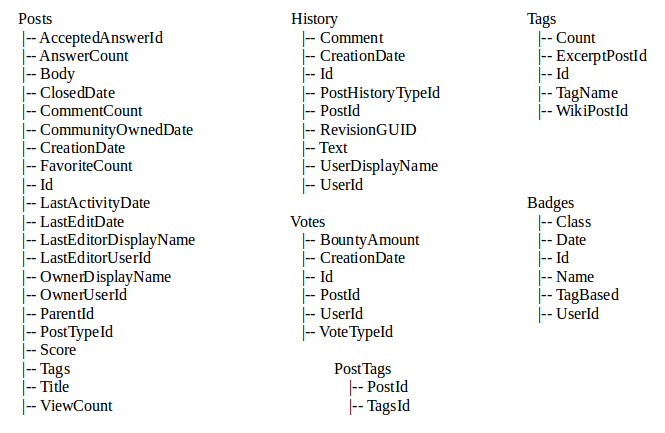
\includegraphics[scale=0.68]{graphics/schema-stack} 
\end{figure}

Llegados a este punto deberemos establecer que datos serán los que utilicemos y qué valor poseen estos. El primer problema al que nos enfrentemos será definir el término ``popularidad''; para ello nos encontramos con varias formas de resolverlo: qué pregunta recibe más votos, cuál recibe más \textit{badges}, cuál es el más visitado, sobre cuál se crean más \textit{posts}, en cuál comenta más gente, etc...

Realizando un pequeño análisis descubrimos varias cosas:
\begin{itemize}
	\item No tenemos información sobre le número de visitas.
	\item Los tipos de votos son demasiado dispares para definir un valor exacto de cada en relación al \textit{tag}.
	\item Los \textit{badges} varían a lo largo del tiempo, asignándose más a principios y finales de año, debido a la naturaleza de los mismos.
	\item Los comentarios no indican el interés absoluto de los profesionales del sector, unicamente la capacidad, conocimiento o participación de los usuarios activos.
	\item Los \textit{posts} se crean cuando los usuarios tienen una duda no resuelta anteriormente o cuando la duda no se resuelve fácilmente.
\end{itemize}

Este sencillo análisis deja solamente una opción dirigida directamente a resolver los \textit{insights} establecidos, los \textit{posts}.

Una vez que hemos decidido que serán los \textit{posts} quienes no  van a proporcionar los datos necesarios para resolver la popularidad, continuaermos analizando cuáles de estos datos serán los más relevantes. 

Los datos que a \textit{priori} consideramos más relevantes son el \textit{tag}, el \textit{creationDate} y el \textit{score}. Además, para obtener el \textit{tag} de cada \textit{post}, deberemos cruzarlos con la tabla de \textit{tags} a través de \textit{PostTags}, que nos permitirán conocer que lenguaje o tecnología pertenece cada \textit{posts}.

Realizaremos una primera consulta a través del módulo de \textit{Spark SQL} y almaceno los resultados. En el fragmento de código \ref{stof:anaTopSQL} podemos ver como se realiza una consulta a través de este módulo. Pero de momento la consulta \gls{SQL} usada para la relación se puede observar en fragmento de código \ref{stof:sql1}.

% Escribir código 
\begin{lstlisting}[label=stof:sql1,language=sql,frame=single,caption={Consulta \gls{SQL} para la extraccion de la fecha, \textit{tag} y \textit{score} de las consultas en \textit{Stack Overflow}.}]
SELECT t.tag,
	date_format(creation_date, '%Y-%m) AS month,
	COUNT(*) AS count,
	SUM(q.score) AS score
FROM posts p
INNER JOIN tags t on p.id = t.id
WHERE score > 0
GROUP BY month, t.tag;
\end{lstlisting}

La consulta del código \ref{stof:sql1} nos devolverá la puntuación que le han dado los usuarios ordenada por mes y lenguaje, almacenamos los datos, para análisis futuros. A partir de estos datos, podemos realizar la búsqueda de los lenguajes más populares.

Establecemos una búsqueda de los lenguajes atendiendo al número de apariciones de los lenguajes en el último año, a través de \textit{Spark SQL}.
Estas consultas son gestionadas por el \textit{Spark Core}. Para empezar a trabajar con \textit{Apache Spark} debemos declarar algunas variables importantes como son el \textit{SparkContext} o el \textit{SparkSession}.

En primer lugar, realizaremos los \textit{imports} y la inicialización tanto de \textit{SparkContext}, como del \textit{SparkSession} tal y como se puede apreciar en el fragmento de código \ref{stof:anaImport}, esto será común a todos los scripts de \textit{Apache Spark} por lo que se evitará repetir código a lo largo del proyecto.

\begin{lstlisting}[label=stof:anaImport,language=Python,frame=single,caption=\textit{Imports} y configuración de una sessión de \textit{Apache Spark}.]
from pyspark import SparkConf, SparkContext
from pyspark.sql.functions import col, asc, desc
from pyspark.sql.types import StructType, StructField, StringType, IntegerType

conf = SparkConf().setAppName("Jupyter: Stack Posts")
conf = conf.setMaster("spark://david-hdp:7077")
sc = SparkContext(conf=conf)
spark = SparkSession(sc)
\end{lstlisting}

Dado que los resultados del código \ref{stof:sql1} se han exportado a un \gls{CSV} sin cabecera, deberemos crear un \textit{schema} de manera manual, para ello \textit{Apache Spark} proporciona unos tipos de datos propios para relacionas los \textit{schemas} con su origen de datos. Como se puede observar en el código \ref{stof:anaSchema}, se ha creado un \textit{schema} de cuatro campos.

\begin{lstlisting}[label=stof:anaSchema,language=Python,frame=single,caption=Código de declaración del \textit{schema} para lectura del \gls{CSV}.]
schema = StructType([
	StructField("tag", StringType(), True),
	StructField("fecha", StringType(), True),
	StructField("count", IntegerType(), True),
	StructField("score", IntegerType(), True),
	StructField("answers", IntegerType(), True)])
\end{lstlisting}

El siguiente paso será importar el fichero que contiene los datos indicandole el \textit{schema} del fragmento de código \ref{stof:anaSchema} y lo guardamos en una variable llamada ``df'' de la forma que aparecen el código \ref{stof:anaDF} y posteriormente se visualiza una muestra de los datos para comprobar como están almacenados los datos. Esta muestra se puede ver en la tabla \ref{stof:dfTable} donde vemos los $6$ primeros elementos del \textit{dataframe}.

\begin{lstlisting}[label=stof:anaDF,language=Python,frame=single,caption=Carga de un fichero \gls{CSV} con un esquema predefinido con el módulo \textit{Spark \gls{SQL}}.]
df = spark.read.csv('stof/clean/mysql_clean.csv', schema=schema)
\end{lstlisting}

\begin{table}[htp!]
	\centering
	\caption{\textit{DataFrame} de muestra de datos de \textit{Stack Overflow}.}
	\label{stof:dfTable}
	\begin{tabular}{@{}|r|r|r|r|r|@{}}
		\hline
		\textbf{tag}  & \textbf{fecha}   & \textbf{count} & \textbf{score} & \textbf{answers} \\ \hline
		.net & 2010-03 & 1073  & 6385  & 2768    \\
		.net & 2011-02 & 1036  & 4408  & 2101    \\
		.net & 2011-03 & 1030  & 5493  & 2192    \\
		.net & 2010-08 & 1018  & 5003  & 2443    \\
		.net & 2011-05 & 1004  & 4015  & 1906    \\
		.net & 2011-04 & 987   & 3718  & 1977    \\ 
		\hline
	\end{tabular}
\end{table}

Una vez que tengamos los datos cargados, ya se puede empezar a trabajar con ellos. El primer hito a resolver son los lenguajes más populares. Para ello vamos a realizar una consulta \gls{SQL} que nos devuelva los diez primeros lenguajes y/o tecnologías más populares del último año. El primer paso será generar una tabla temporal para poder operar con \gls{SQL}, dicha función la cumple la primera línea del fragmento de código \ref{stof:anaTopSQL}.

\begin{lstlisting}[label=stof:anaTopSQL,language=Python,frame=single,caption=Código de generación de la tabla temporal y la ejecución de una consulta \gls{SQL}.]
# Nueva tabla temporal
df.createOrReplaceTempView("temp_talble")

# Ejecucion de consulta SQL
top10 = spark.sql("\
	SELECT tag, \
		SUM(count) AS count, \
		SUM(score) AS score\
	FROM temp_table \
	WHERE \
		fecha >= "2016-12" \
	GROUP BY tag \
	ORDER BY count DESC \
	LIMIT 10")
\end{lstlisting}

El resultado de esta consulta se muestra en la tabla \ref{stof:anaTop}, esta es la lista de las diez tecnologías más populares o, dicho de otra manera, sobre qué tecnologías están preguntando los profesionales del sector de \gls{IT}. 

\begin{table}[htp!]
	\centering
	\caption{Tabla con los 10 lenguajes más populares de \textit{Stack Overflow}.}
	\label{stof:anaTop}
	\begin{tabular}{|r|r|r|}
		\hline
		\multicolumn{1}{|c|}{\textbf{tag}} & \multicolumn{1}{c|}{\textbf{count}} & \multicolumn{1}{c|}{\textbf{score}} \\ \hline
		javascript                         & 482970                              & 876320                              \\
		c\#                                & 436792                              & 810352                              \\
		java                               & 354105                              & 644255                              \\
		android                            & 352392                              & 720040                              \\
		python                             & 267364                              & 498320                              \\
		c++                                & 232816                              & 677424                              \\
		php                                & 213584                              & 328408                              \\
		ios                                & 181032                              & 383838                              \\
		c                                  & 91936                               & 219344                              \\
		\multicolumn{1}{|r|}{html}         & \multicolumn{1}{c|}{91788}          & \multicolumn{1}{c|}{163830}         \\ \hline
	\end{tabular}
\end{table}

Con estos datos se puede iniciar el aprovisionamiento de datos en twitter utilizando estos resultados como \textit{keywords}.
